\documentclass[aps,prl,reprint,amsmath,amssymb,floatfix]{revtex4-2}

\usepackage{graphicx}
\usepackage{bm}
\usepackage{amssymb}
\usepackage{amsmath}
\usepackage{physics}
\usepackage[colorlinks=true,linkcolor=blue,citecolor=blue,urlcolor=blue]{hyperref}

\newcommand{\hsys}{H_{\text{sys}}}
\newcommand{\hf}{H_{F}}
\newcommand{\UK}{U_{\text{K}}}
\newcommand{\UI}{U_{\text{I}}}
\newcommand{\Usys}{U_{F}[\bm{h}]}
\newcommand{\HK}{H_{\text{K}}}
\newcommand{\HI}{H_{\text{I}}}
\newcommand{\EN}{E_{\mathcal N}}
\newcommand{\ENinf}{E_{\mathcal N}^{\infty}}
\newcommand{\Psym}{P_{\rm sym}}

\begin{document}

\title{Symmetry fixes the entanglement floor in a correlated environment (working title)}

\author{Bhavay Tyagi}
\email{btyagi@uh.edu}
\affiliation{Department of Physics, University of Houston, Houston, Texas 77204, USA}
\author{Eric R. Bittner}
\affiliation{Department of Physics, University of Houston, Houston, Texas 77204, USA}
\author{Kevin E. Bassler}
\affiliation{Department of Physics, University of Houston, Houston, Texas 77204, USA}
\date{\today}

\begin{abstract}
%A bath destroys only what it can resolve. We drive a kicked Ising ring with
%noise correlated across sites with strength $\xi$. The half-chain negativity
%then reaches exactly zero at a time $A/(1-\xi)$, predicted out of sample to
%$0.2\,\%$. At $\xi=1$ it stops instead at a floor---the maximally mixed state
%on the ring-symmetric subspace---which has a closed form, does not depend on
%the dissipation rate, lies below $\log 2L$, is the same for every
%ring-symmetric initial state including the unentangled $\ket{0\cdots0}$, and is
%removed by any site-to-site disorder.
\end{abstract}

\maketitle

{\it Introduction}---We traditionally treat noise as the enemy of coherence, and typical solutions include isolating
the system better, or correct its errors~\cite{Acharya2023}. Most treatments overlook a third solution: what can
the environment actually \emph{see}? An environment destroys only what it can resolve. A bath connected to $L$ qubits through $L$
independent quantum channels resolves each qubit separately, and can damage any degree
of freedom the system possesses. However, a bath connected through one shared mode
sees only a weighted sum, or the total spin for equal couplings~\cite{Blais2021}. Spatial correlation makes an environment partially blind. Spatially correlated noise can dominate the dephasing
of trapped-ion registers~\cite{Kielpinski2001,Langer2005,Monz2011,Dasu2025},
and experiments measure it directly for superconducting
qubits sharing an engineered source~\cite{vonLupke2020} and for silicon spin
qubits~\cite{Yoneda2023}, and in principle from single-qubit operations
alone~\cite{Gulacsi2025}. Decoherence-free subspaces and noiseless subsystems
store information in states a collective bath cannot
distinguish~\cite{Zanardi1997,Lidar1998,Knill2000}, and
experiments confirm them in ions~\cite{Kielpinski2001,Langer2005},
photons~\cite{Kwiat2000} and NMR~\cite{Viola2001}. In these scenarios, one typically prepares the states in advance, and engineers the dynamics to keep them protected. Our earlier work, however, needed no such design, we
showed that collective behavior such as synchronization, induced by a shared correlated environment for two coupled
spins~\cite{Tyagi2024} and for oscillators sampled from random initial
conditions~\cite{Bittner2025jcp}, can protect quantum resources and aid coherent transport.

 \emph{In this letter} we extend
that question to a many-body system and ask what a correlated bath does to the
entanglement generated by the dynamics of a chaotic driven chain.
The correlation $\xi$, the fraction of each qubit's noise power shared with
every other, sets how much the bath can see. At $\xi=0$ the $L$ noise channels
are independent, and at $\xi=1$ a single channel is common to all of them.
There is no critical value of $\xi$. In the limit $\xi\to1$ the entanglement
\emph{lifetime} diverges as $(1-\xi)^{-1}$, while the negativity still reaches
exactly zero at a finite time for every $\xi<1$. Only at $\xi=1$ does the decay
stop, at a nonzero floor we obtain in closed form from the ring's symmetry
group [Fig.~\ref{fig:model}], with no dynamics and no dependence on the
dissipation rate. The internal dynamics of the model builds the entanglement,
and the bath fixes how much of it survives.

\begin{figure}[t]
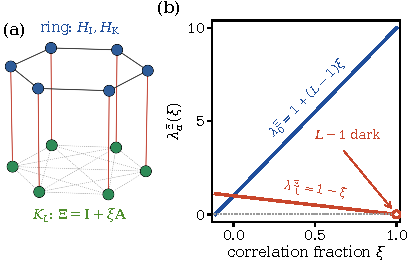
\includegraphics[width=\linewidth]{Figures/fig1_model}
\caption{\label{fig:model}%
(a) The Hamiltonian~\eqref{eq:SysHam} lives on a ring (top); we choose the bath-correlation graph (bottom) independently of it, and is here
$K_L$. Vertical links are the local system--bath couplings. (b) Eigenvalues of
$\bm\Xi(\xi)$ for $K_L$ at $L=10$: the uniform mode brightens as $1+(L-1)\xi$
while the $L-1$ relative modes, degenerate at $1-\xi$, go dark together at
$\xi=1$.}
\end{figure}

{\it Model}---The system is the self-dual kicked Ising ring, a minimal locally
interacting model of many-body quantum chaos~\cite{Bertini2018,Bertini2019},
\begin{align}
\label{eq:SysHam}
\hf[\bm h;t] &= \HI[\bm h]+\sum_{m\in\mathbb Z}\delta(t-m)\,\HK ,\\
\HI &= J\sum_{j=1}^{L}\sigma^z_j\sigma^z_{j+1}+\sum_{j=1}^{L}h_j\sigma^z_j ,
\qquad
\HK = b\sum_{j=1}^{L}\sigma^x_j , \nonumber
\end{align}
with periodic boundary conditions, so the one-period Floquet operator is
$U_F[\bm h]=e^{-i\HK}e^{-i\HI[\bm h]}\equiv\UK\UI$. We work at the self-dual
point $|J|=|b|=\pi/4$, where the model is exactly solvable and described by a dual-unitary circuit~\cite{BertiniClaeysProsen2026}, its
quantum-chaotic spectral statistics for $\bm h\neq0$ have been established
exactly~\cite{Bertini2018}, and a class of product states (``class
$\mathcal T$'') has exactly solvable entanglement growth~\cite{Bertini2019}.
Numerics use $h_j=h=1$ and the class-$\mathcal T$ state $\ket{+}^{\otimes L}$.
%(Our code uses the equivalent kick angle $b=-\pi/4$; the two Floquet operators
%are complex conjugates, so $\rho^{T_A}$ has the same spectrum.)

The ring couples to a bath whose local noise channels are not independent,
through a Gorini--Kossakowski--Sudarshan--Lindblad
generator~\cite{Lindblad1976,Gorini1976,Breuer2007} with site-basis dissipator
\begin{equation}
\label{eq:dissipator_site}
\mathcal L^{(\xi)}_{\rm diss}[\rho]=\sum_a\gamma_a\!\!\sum_{i,j=1}^{L}\!\!
\Xi_{ij}(\xi)\Bigl[\ell^{(a)}_i\rho\,\ell^{(a)\dagger}_j
-\tfrac12\bigl\{\ell^{(a)\dagger}_j\ell^{(a)}_i,\rho\bigr\}\Bigr],
\end{equation}
where $a$ labels the microscopic process: $\ell^{(z)}_j=\sigma^z_j$ for
collective dephasing, the channel we lead with, and
$\ell^{(-)}_j=\sigma^-_j$ (or both $\sigma^\mp_j$ with rates
$\gamma_\mp=\gamma(n_{\rm th}+\tfrac12\pm\tfrac12)$ at finite temperature) for
amplitude damping. The noise-correlation matrix is
$\bm\Xi(\xi)=\mathbf I+\xi\mathbf A$, with $\mathbf A$ the adjacency matrix of
a \emph{bath-correlation graph} chosen independently of the ring the
Hamiltonian lives on (Fig.~\ref{fig:model}). Since $\bm\Xi$ is a polynomial in
$\mathbf A$ it shares its eigenvectors $v_\alpha$ and has eigenvalues
$\lambda^\Xi_\alpha=1+\xi\lambda_\alpha$, so
Eq.~\eqref{eq:dissipator_site} becomes a sum of independent collective channels
with jump operators $\ell^{(a)}_\alpha=\sum_jv_\alpha(j)\ell^{(a)}_j$ and
weights $\gamma_a\lambda^\Xi_\alpha\ge0$~\cite{SM}; a channel goes \emph{dark}
when its weight vanishes. For $K_L$, $\mathbf A=\mathbf J-\mathbf I$ has two
eigenvalues, $\lambda_0=L-1$ for the uniform mode and $\lambda_\perp=-1$ with
multiplicity $L-1$, so that
\begin{equation}
\label{eq:complete_graph_split}
\mathcal L^{(\xi)}_{\rm diss}=\bigl[1+(L-1)\xi\bigr]\mathcal D_0
+(1-\xi)\,\mathcal D_\perp ,
\end{equation}
where $\mathcal D_0$ is the dissipator of the uniform jump operator
$\ell^{(a)}_0=L^{-1/2}\sum_j\ell^{(a)}_j$ and $\mathcal D_\perp$ the sum of the
$L-1$ relative ones, and $\bm\Xi(\xi)$ is positive semidefinite precisely on
$-1/(L-1)\le\xi\le1$. At $\xi=1$ all $L-1$ relative channels vanish at once,
$\operatorname{rank}\bm\Xi$ collapses from $L$ to $1$, and the one surviving
jump operator is collective: $J^z$ for dephasing, $J^-$ (and $J^+$) for
amplitude damping.

For dephasing, Eq.~\eqref{eq:dissipator_site} is not an approximation but the
\emph{exact} average of the unitary dynamics over classical Gaussian phase
noise with covariance $\gamma\bm\Xi$, carrying no weak-coupling assumption at
any $\gamma$ or $L$ (Appendix). That makes $\Xi_{jk}$ a measurable Pearson
coefficient rather than a modeling choice, and makes $\xi=1$ a statement about
one shared noise line rather than fine tuning [Eq.~\eqref{eq:onenoiseline}].
Amplitude damping admits no such derivation: those are genuine quantum-bath
channels, with the usual Born--Markov conditions and collective rate $L\gamma$
as the small parameter ($0.1$ here)~\cite{SM}.

We follow the entanglement across a bipartition $A|A^c$, $A=\{1,\dots,N_A\}$,
with the logarithmic negativity
$\EN(\rho)=\log\lVert\rho^{T_A}\rVert_1=\log(1+2\mathcal N)$, $\mathcal N$
being the sum of the absolute values of the negative eigenvalues of
$\rho^{T_A}$~\cite{Peres1996,Horodecki1996,Vidal2002,Plenio2005}. For a
globally pure state this equals the R\'enyi-$1/2$ entropy of
$\rho_A$~\cite{SM}, and in the closed system it gives the class-$\mathcal T$
baseline $\EN(t)=\min(2t,N_A)\log2$---a thermodynamic-limit statement valid
only while the light cone has not wrapped the ring, $2t\le\min(N_A,N_B)$. Over
the ten points at $L=10$ inside that window our closed evolution reproduces it
to $1.1\times10^{-14}$~\cite{SM}. We use the stroboscopic map
$\mathcal M_\xi=e^{\mathcal L^{(\xi)}_{\rm diss}}\circ\mathcal U_F$, in which
the bath acts once per period.

\begin{figure}[t]
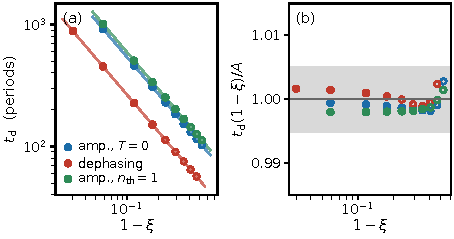
\includegraphics[width=\linewidth]{Figures/fig2_lifetime_r2}
\caption{\label{fig:lifetime}%
The lifetime law, $L=10$, $N_A=5$, $\gamma=10^{-2}$ ($3\times10^{-3}$,
$n_{\rm th}=1$ for the finite-temperature channel). (a) Death time against
$1-\xi$; open symbols are the calibration set chosen by the prediction-blind
criterion in the text, we predicted the filled symbols from the lines $A/(1-\xi)$
before being computed. (b) The same data as $t_d(1-\xi)/A$, band $\pm0.5\,\%$.
Largest out-of-sample error: $0.17$, $0.16$, $0.20\,\%$, in legend order.}
\end{figure}

{\it The lifetime diverges}---For every $\xi<1$ the negativity reaches
\emph{exactly} zero at a finite time and stays there
($\lvert\EN\rvert\le4.4\times10^{-16}$ thereafter). This is entanglement sudden
death~\cite{Yu2004,Yu2009}, and for dephasing it is forced rather than
accidental: at any $\xi<1$ that map is unital and its Kraus algebra contains
every $\sigma^z_j$ together with $U_F$, so the unique fixed point is
$\openone/2^L$, which lies in the \emph{interior} of the
positive-partial-transpose set, and a trajectory converging to it must enter
that interior after a finite time~\cite{SM}. The negativity therefore vanishes
\emph{linearly} at the death time, and a decay rate fitted inside a fixed
window of $\EN$ values inherits the window rather than the
dynamics~\cite{SM}. The parametrization-free observable is the death time
itself, and it obeys
\begin{equation}
\label{eq:lifetime}
t_d(\xi)=\frac{A}{1-\xi}\bigl[1+O(1-\xi)\bigr] .
\end{equation}

How we tested this matters, because Eq.~\eqref{eq:lifetime} is asymptotic in
$1-\xi$, so a calibration set needs a rule. We use one that never looks at a
prediction point: from adjacent pairs form the local exponent
$q=\Delta\log t_d/\Delta\log(1-\xi)$, declare the asymptotic regime to begin at
the largest $1-\xi$ beyond which every subsequent $q$ lies within $0.05$ of
$-1$, and calibrate $A$ as the mean of $t_d(1-\xi)$ over the points inside that
regime that are reachable in the original $150$-period window; everything at
higher $\xi$ is a prediction. At $L=10$ this gives $A=26.441$ (dephasing),
$53.810$ and $59.080$ (zero- and finite-temperature amplitude damping) periods,
and the predicted death times are then correct to a maximum of $0.16\,\%$,
$0.17\,\%$ and $0.20\,\%$ over four, six and six out-of-sample points spanning
a sevenfold extrapolation in lifetime [Fig.~\ref{fig:lifetime}]. Free-exponent
fits inside the regime give $-1.0006$, $-0.9997$ and $-0.9989$ against the
predicted $-1$, and independently the spectral gap of the one-period
map---which refers to no entanglement measure at all---is linear in $1-\xi$ to
$0.12\,\%$, $0.37\,\%$ and $0.94\,\%$ at $L=4$, $6$ and $8$~\cite{SM}.

Three qualifications belong with them. The quoted $A$ are properties
of the stroboscopic map, of the stated $L$ and $\gamma$, and of one death-time
convention, $t_d$ being the last log-interpolated crossing of $\EN=10^{-3}$:
moving to $\EN=10^{-2}$ or to the algebraic condition $\rho^{T_A}\succeq0$
shifts $A$ by up to $35\,\%$ (dephasing: $20.83$ to $28.06$) while the exponent
stays within $0.004$ of $-1$ under every convention, which enters only a
$\xi$-independent numerator~\cite{SM}. $A$ also grows with size---$20.20$,
$25.14$, $26.44$ at $L=6,8,10$---by $24\,\%$ and then $5\,\%$, and the
Supplemental Material derives $\gamma A\to\log2/2$, so it saturates. Finally,
there is no threshold: an apparent onset of protection near $\xi\approx0.65$ is
where $t_d$ crosses the end of a $150$-period run.

\begin{figure}[t]
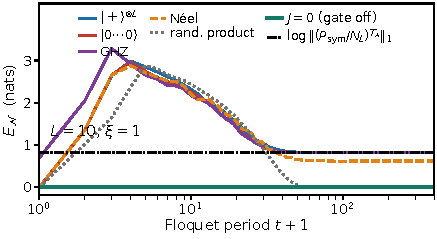
\includegraphics[width=\linewidth]{Figures/fig3_basin}
\caption{\label{fig:basin}%
Collective dephasing at $\xi=1$, $L=10$, $\gamma=10^{-2}$, $N_A=5$.
$\ket{+}^{\otimes L}$, $\ket{0\cdots0}$ and a GHZ state all reach the closed
form~\eqref{eq:fixed_point} (dot-dashed) to $\le1.5\times10^{-14}$, from above,
after the drive has raised $\EN$ to $\simeq3$ nats. The N\'eel state, invariant
under only half of $D_L$, freezes lower; a random product state dies; with the
entangling gate removed ($J=0$) the negativity is identically zero.}
\end{figure}

{\it The floor, in closed form}---At $\xi=1$ the behavior is qualitatively
different: over $2000$ Floquet periods the dephasing drift of $\EN$ on the last
$500$ is $-2.6\times10^{-19}$ per period, peak to peak $1.1\times10^{-15}$
nats. The entanglement freezes; it does not slowly decay.

For collective dephasing we can write the frozen state down exactly. The
surviving jump operator $L_z=2\sqrt\gamma J^z$ is Hermitian and diagonal, so
the one-period map is unital and its fixed points form the commutant of the
algebra generated by its Kraus operators~\cite{Kribs2003,Arias2002}. That
algebra is $\operatorname{alg}\{U_F,J^z\}$ for \emph{every} $\gamma>0$, which
proves that the frozen state cannot depend on the dissipation rate.
Identifying the commutant with the ring symmetry gives
\begin{equation}
\label{eq:fixed_point}
\rho_\infty=\frac{\Psym}{N_L} ,
\qquad
\ENinf=\log\bigl\lVert(\Psym/N_L)^{T_A}\bigr\rVert_1 ,
\end{equation}
where $\Psym=\lvert G\rvert^{-1}\sum_{g\in G}U(g)$ projects onto the states
invariant under the full ring symmetry group $G=D_L$ ($L$ rotations, $L$
reflections) and $N_L=\Tr\Psym$ is the number of binary \emph{bracelets} of
length $L$: $N_L=6,13,30,78,224$ for $L=4,6,8,10,12$. The derivation, and the
one genericity hypothesis it rests on---the irreducibility of an explicit pair
of $N_L\times N_L$ matrices, which we verify directly at $L=4,\dots,12$---are
in the Appendix. Equation~\eqref{eq:fixed_point} involves no time evolution,
yet at $L=10$ its value $0.823820166737$ agrees to $4\times10^{-14}$ with a
$2000$-period evolution through an independent propagator, and at $L=6,8,10$
the dephasing plateau equals it to all twelve quoted digits at every $\gamma$
from $3\times10^{-3}$ to $0.1$. Because it requires the exact $D_L$ symmetry,
any site-to-site spread of the Hamiltonian removes the floor entirely; we
quantify below how slowly.

Equation~\eqref{eq:fixed_point} is a statement about collective
\emph{dephasing}. Zero-temperature amplitude damping has no closed form,
because its map is not unital; its plateau sits $1.70\,\%$ above the dephasing
value at $L=10$ and moves by $8.8\,\%$ over a factor $10$ in $\gamma$
(Appendix). Those are two channels, not two values of one number.

Because $\rho_\infty$ is an equal mixture of $N_L$ cat states, one over each
$G$-orbit of computational basis states, and a pure state of Schmidt rank $r$
has $\lVert\psi^{T_A}\rVert_1\le r$ while every orbit has size at most
$\lvert G\rvert=2L$, convexity gives the exact bound $\ENinf\le\log2L$: the
floor grows at most logarithmically with $L$ and is not extensive. In absolute
terms it is $1.19$ ebits at
$L=10$ and $1.49$ at $L=14$, against a bound of $4.32$ and $4.81$---a little
more than one Bell pair across ten to fourteen qubits, carried by a rank-$N_L$
mixed state. A $\log L$ result of this size is worth reporting because it is exact and
closed, not because the amount is large. Its area law has a cost: the floor is
flat in block size rather than a Page curve---at $L=10$ it varies by $6\,\%$
over every contiguous block $2\le N_A\le8$ while $\min(N_A,N_B)\log2$ varies by
a factor $2.5$---because it is one global object seen the same way by every
cut~\cite{SM}, and so is invisible to any few-body probe.

{\it Symmetry, not scrambling}---Equation~\eqref{eq:fixed_point} says where the
floor comes from. The fully correlated bath contributes exactly one element to
the conserved algebra, $J^z$; everything else in
$\operatorname{alg}\{U_F,J^z\}'$ is the symmetry of the Hamiltonian. Three
tests confirm this. The floor does not change at $h=0$, the \emph{integrable}
point, so it is not a diagnostic of chaos. A site-dependent longitudinal field
destroys the ring symmetry and collapses it to exactly zero
($\ENinf=-2\times10^{-16}$ at $L=6,8$ for random $h_j$), while a partial
symmetry gives a reduced value ($0.182$ at $L=6$, $0.357$ at $L=8$ for a
period-two field). And dense connectivity of the bath graph is not enough:
circulant $k$-regular correlation graphs at $L=10$, sampled at $\xi=0.5$, $0.9$
and $1.0$ of their positivity endpoints, give a late-time negativity zero to
$10^{-13}$ for $k=2,4,6,8$; a floor appears only at $k=9=L-1$, where
$\operatorname{rank}\bm\Xi=1$.

The same algebra fixes the physical reading. Because $\Psym$ commutes with
$U_F$ and with $J^z$, the isotypic weights $w_\lambda=\Tr(\Pi_\lambda\rho)$ of
$D_L$ are exact constants of the motion (drift $1.6\times10^{-14}$ over $1500$
periods) and $\rho_\infty$ lives entirely in the trivial component, so the
basin of attraction of Eq.~\eqref{eq:fixed_point} is \emph{exactly} the states
with $w_{A_1}=1$ and nothing larger. Inside it the floor does not remember the
initial condition: $\ket{+}^{\otimes L}$, the unentangled $\ket{0\cdots0}$, a
GHZ state and a $W$ state all arrive at the same value to
$\le1.5\times10^{-14}$ at $L=6,8,10$, from above and from below
[Fig.~\ref{fig:basin}]. Outside it they do not: the N\'eel state, invariant
under only $L$ of the $2L$ elements of $D_L$, has $w_{A_1}=\tfrac12$ exactly
and freezes at $0.622$ at $L=10$, while Haar-random, random-product and
maximally mixed states never reach $\rho_\infty$. The dual-unitary structure
still fixes the maximal early growth that loads entanglement into the state,
but it does not set the floor.

{\it Experimental reach}---$A$ is inversely proportional to the dephasing rate
($\gamma A$ varies by $1\,\%$ over a factor $33$ in $\gamma$), so
Eq.~\eqref{eq:lifetime} has a device-independent form: with $T_2=1/2\gamma$ for
a single qubit,
\begin{equation}
\label{eq:tdT2}
\frac{t_d}{T_2}=\frac{2\gamma A}{1-\xi}\simeq\frac{0.56}{1-\xi}
\qquad(L=10,\ \rho^{T_A}\succeq0),
\end{equation}
$0.42$ and $0.52$ at $L=6$ and $8$, rising towards the derived asymptote
$\log2$ (Appendix). The Floquet period has cancelled: the floor persists for
$\simeq0.56/(1-\xi)$ \emph{single-qubit dephasing times} on any platform, and
preparing it from $\ket{0\cdots0}$ costs about one~\cite{SM}.

For $\xi$ itself there is a number from a real device. At $L=2$ a single-ion
superposition dephases at $2\gamma$ and a decoherence-free-subspace state at
$4\gamma(1-\xi)$, so $1-\xi=\tfrac12\Gamma_{\rm DFS}/\Gamma_{\rm test}$.
Kielpinski \emph{et al.}~\cite{Kielpinski2001} measured that pair on two
$^9$Be$^+$ ions under a \emph{deliberately applied} common-mode source and
found $0.0035\pm0.0050$ against $0.18\pm0.01\,$ms$^{-1}$. The numerator is
consistent with zero, so this is a bound and not a value: $1-\xi<0.024$ at
$1\sigma$, a floor lasting more than twenty-three single-qubit dephasing times.
Their \emph{ambient} numbers give only $1-\xi\lesssim0.14$. Where $\xi$ has
been measured rather than bounded is the silicon spin-qubit pair of
Ref.~\cite{Yoneda2023}, whose $\Xi_{12}\approx0.7$ implies $t_d\approx1.9\,T_2$:
enough to resolve a floor, not to freeze one. Trapped ions remain the natural
host, since a global field fluctuation or beam is literally the shared line of
Eq.~\eqref{eq:onenoiseline}, $\xi$ is tunable through the beam intensity, and
kicked-Ising Floquet dynamics has been run there for hundreds of
periods~\cite{Kyprianidis2021}.

The binding constraint is not $\xi$ but uniformity. Three imperfections act in
parallel, so their rates add; at $L=10$, per Floquet period, in one death-time
convention,
\begin{equation}
\label{eq:budget}
t_{\rm obs}^{-1}\simeq\frac{\gamma(1-\xi)}{0.26}+\frac{w_h^2}{1.7}
+\frac{\gamma\,w_g^2}{1.3},
\end{equation}
with $w_h$ the relative site-to-site spread of the longitudinal field and $w_g$
that of the coupling to the shared noise line. The second coefficient is
$t_dw_h^2=1.7$, from $41$ disorder realizations per cell at $L=6,8$, with cell
medians $1.2$--$2.6$ and no significant size dependence~\cite{SM}. Equating the first two terms gives
$w_h\lesssim2.5\sqrt{\gamma(1-\xi)}$ against $w_g\lesssim2.2\sqrt{1-\xi}$, i.e.\
$w_h\lesssim2.5\,\%$ but $w_g\lesssim22\,\%$ at $\gamma=10^{-2}$ per period and
$1-\xi=10^{-2}$. Only the disorder term is independent of $\gamma$, because it
acts through the unitary at second order in $w$: a quieter device needs a more
uniform one. Superconducting processors already run Floquet circuits of this
three-layer form past a hundred cycles on twenty qubits, but with random rather
than uniform fields and couplings on an open chain~\cite{Mi2022}: the
uniformity a ring symmetry needs is exactly what they lack.

Reading the floor out needs the whole ring, since no contiguous block of up to
six sites is entangled at $L=10$~\cite{SM}. The \emph{mechanism} is cheap: the
$2L$ permutation expectations $\langle U(g)\rangle$ equal unity on
$\rho_\infty$ and on $\ket{0\cdots0}$, and their decay calibrates the disorder
term of Eq.~\eqref{eq:budget} \emph{in situ} at $O(10^2)$ shots~\cite{SM}.
They are not entanglement witnesses---$\ket{0\cdots0}$ saturates them---and
must accompany an entanglement measurement, not replace it.

{\it Discussion}---A correlated bath cannot create entanglement, but it can
decide how much is left. Away from $\xi=1$ it buys a lifetime diverging as the
inverse of the residual independent-noise fraction; at $\xi=1$ it buys a floor
the ring symmetry fixes. That floor is a passive quantum memory of one
collective degree of freedom, not a route to extensive protected
entanglement.

Read the other way, the same law is a measurement: because $t_d$ diverges as
$\xi\to1$, a many-body entanglement lifetime probes a small independent-noise
fraction far more sensitively than the two-qubit observables normally used. At
$\xi=0.90$ the superdecoherence exponent moves only from $2.000$ to $1.972$,
while $t_d$ changes by a factor of ten.

We state three limitations plainly. The framework is Markovian
throughout, and we have not tested whether the dark-mode structure survives a
bath with memory on the scale of a Floquet period.
Equation~\eqref{eq:fixed_point} rests on a genericity condition that we verify
directly at $L=4,\dots,12$ but do not prove. And everything here uses $D_L$
because the Hamiltonian is a uniform ring; we have not examined other symmetry
groups and claim no generality beyond the case tested.

\section*{acknowledgments}
This work was supported by the National Science Foundation (CHE-2404788) and
the Robert A. Welch Foundation (E-1337). Claude Opus helped with some numerical calculations and as a writing aid. In memory of Shantanu and Yatharth. 


\section*{Data availability}
We deposit the propagator code, the analysis scripts and the data files
behind every figure and number quoted here as a single public archive, whose
DOI will appear in the published version.

\bibliographystyle{apsrev4-2}
\bibliography{References_local}

\clearpage
\section*{Appendix}

\paragraph*{Derivation of the fixed point.}
At $\xi=1$ the only surviving dephasing jump operator is
$L_z=\sqrt{\gamma}\sum_j\sigma^z_j=2\sqrt{\gamma}J^z$, which is Hermitian and
diagonal, so the dissipative step is exactly a multiplicative damping of the
magnetization coherences,
$(\Phi_\gamma X)_{ab}=e^{-2\gamma(m_a-m_b)^2}X_{ab}$, and the one-period map
$\mathcal M_1=\Phi_\gamma\circ\mathcal U_F$ is unital. $\Phi_\gamma$ is a
random-phase channel,
$\Phi_\gamma(X)=\int d\varphi\,p(\varphi)e^{-i\varphi L_z}Xe^{i\varphi L_z}$
with $p$ Gaussian, so $\mathcal M_1$ has Kraus operators
$K_\varphi=\sqrt{p(\varphi)}e^{-i\varphi L_z}U_F$. The kernel
$G_{mm'}=e^{-2\gamma(m-m')^2}$ is strictly positive definite on the $L+1$
distinct magnetizations for every $\gamma>0$, so those Kraus operators span the
whole algebra of operators diagonal in $J^z$ and
\begin{equation}
\label{eq:em_kraus_algebra}
\mathcal A=\operatorname{alg}\{U_F,J^z\}
\qquad\text{for every }\gamma>0 .
\end{equation}
For a unital trace-preserving channel the fixed-point set is the commutant of
the Kraus algebra and the ergodic limit is the trace-preserving conditional
expectation onto it~\cite{Kribs2003,Arias2002}, so
${\rm Fix}(\mathcal M_1)=\mathcal A'$ and
$\rho_\infty=\mathcal E_{\mathcal A'}[\rho(0)]$. Since $\mathcal A$ does not
depend on $\gamma$, neither does $\rho_\infty$: the $\gamma$ independence of
the floor is a proof, not an estimate.

The Hamiltonian is uniform on a ring, so $U_F$ commutes with every element of
$G=D_L$, and every site permutation commutes with $J^z$; hence
$\mathbb C[G]\subseteq\mathcal A'$. For any initial state invariant under $G$
one has $\Tr(U(g)\rho_0)=1$ for all $g$, and because each $U(g)$ is a fixed
point the conditional expectation preserves that value. Since
$\lvert\Tr(U\rho)\rvert\le1$ with equality only if $\rho$ is supported on the
eigenvalue-one eigenspace of $U$,
$\operatorname{supp}\rho_\infty\subseteq\mathcal S=\bigcap_g\ker(U(g)-\openone)$,
whose dimension is the bracelet number $N_L$ by Burnside's lemma.

The remaining step---that $\rho_\infty$ is the \emph{maximally mixed} state on
$\mathcal S$---is the genericity hypothesis. It is not an assumption about the
model as a whole but an irreducibility statement about two explicit
$N_L\times N_L$ matrices: writing $U_S=U_F|_{\mathcal S}$ and
$D_S=J^z|_{\mathcal S}$, Eq.~\eqref{eq:fixed_point} holds for every $\rho_0$
supported on $\mathcal S$ if and only if
$\{X:[X,U_S]=[X,D_S]=0\}=\mathbb C\openone_{\mathcal S}$. A dense singular
value decomposition of the stacked commutator map gives nullity exactly $1$ at
$L=4,6,8,10,12$, with the null singular value at $3$--$7\times10^{-16}$ and the
next one at $0.38$--$0.81$~\cite{SM}. Maximality of a rank is an open condition
in parameters analytic in $(J,b,h)$, so verifying it at one point establishes
it off a proper analytic subvariety. The mean ergodic theorem then gives the
Ces\`aro limit unconditionally, and ordinary convergence follows whenever
$\Tr U_S\neq0$ (measured $0.19$--$0.73$), which excludes the only obstruction, a
quasi-energy spectrum invariant under a rigid rotation of finite
order~\cite{SM}.

\begin{figure}[t]
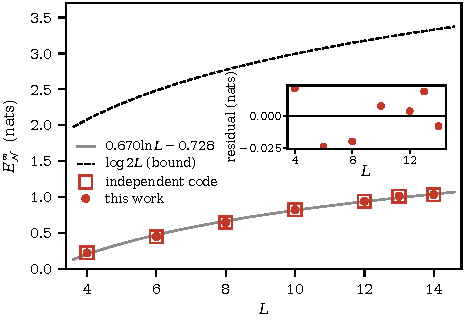
\includegraphics[width=\linewidth]{Figures/fig4_ENinf_L}
\caption{\label{fig:ENinfL}%
The floor against system size, from Eq.~\eqref{eq:fixed_point} with no time
evolution, at the cut $N_A=\lfloor L/2\rfloor$. Filled symbols are our
closed-form values, open symbols an independent implementation at every size. The exact bound
$\ENinf\le\log2L$ is dashed. Inset: residuals to the logarithmic
fit $0.670\log L-0.728$, maximum $0.024$ nats with no systematic trend. A
linear fit to $L\le10$ overshoots the exact $L=12$ and $L=14$ values by $0.094$
and $0.202$ and is excluded.}
\end{figure}

\paragraph*{Size dependence.}
Because Eq.~\eqref{eq:fixed_point} is closed, $\ENinf$ costs one
eigendecomposition of $\Psym^{T_A}$ and no dynamics, which puts $L=14$ within
reach (Fig.~\ref{fig:ENinfL}). The values are $0.2231$, $0.4497$, $0.6465$,
$0.8238$, $0.9420$, $1.0109$ and $1.0336$ nats at $L=4,6,8,10,12,13,14$, with
$N_L=6,13,30,78,224,380,687$. The ratio $\ENinf/\log2L$ is still rising at
$L=14$, so we do not claim an asymptotic coefficient; the bound
$\log2L$ and the exclusion of linear growth are what the data
support.

\paragraph*{Death-time convention.}
$\EN$ reaches exactly zero at $t_d$, and $t_d$ depends on how we declare ``zero''. Two conventions appear here. The \emph{algebraic} one
takes $t_d$ as the exact time at which $\rho^{T_A}\succeq0$; the
\emph{threshold} one takes the last log-interpolated crossing of
$\EN=10^{-3}$, which is what a finite-precision measurement can resolve. They
give the same exponent---the local slope stays within $0.004$ of $-1$ under
either---and differ only in the prefactor. The measured $2\gamma A$ at
$L=6,8,10$ is $0.416$, $0.520$, $0.562$ algebraically and $0.404$, $0.503$,
$0.529$ at threshold, the latter smaller by $3$, $3$ and $6\,\%$.

The distinction matters for one claim. The
Supplemental Material derives $\gamma A\to\log2/2$, that is
$2\gamma A\to\log2=0.693$, as $L\to\infty$. The parameter-free increment test
reproduces that analytic result in the algebraic convention, rising by $0.682$
and $0.693$ over the two available steps in $L$, but it does not at threshold,
where the same increments are $0.658$ and $0.614$ and are falling.
Equation~\eqref{eq:tdT2} is therefore quoted algebraically, the convention in which we derive its asymptote. Three sizes cannot decide whether the
threshold shortfall is a finite-size effect or a property of the threshold
definition itself. The experimentally accessible number is the threshold one,
and it is the smaller of the two.

\paragraph*{Provenance of the dephasing model.}
Equation~\eqref{eq:dissipator_site} usually comes from a weak-coupling Born--Markov reduction. For dephasing that route is unnecessary. Let the ring
evolve under $H(t)=H_S(t)+\sum_jb_j(t)\sigma^z_j$ with $b$ jointly Gaussian,
$\langle b_j(t)b_k(t')\rangle=\gamma\Xi_{jk}\delta(t-t')$. Writing the noise as
a multivariate Wiener process, converting the Stratonovich equation to It\^o
and applying the It\^o product rule to $\rho=\ket{\psi}\bra{\psi}$ returns
Eq.~\eqref{eq:dissipator_site} \emph{identically}: no Born factorization (there
is no bath state), no weak-coupling expansion (it holds to all orders in
$\gamma$), and the only Markov assumption is that the \emph{classical} process
is white over the qubits' response bandwidth, which is a measurable property of
the noise source~\cite{SM}. Three things follow. Since
$\gamma\Xi_{jk}=\langle b_jb_k\rangle$ while $\Xi_{jj}=1$ merely defines
$\gamma$, $\Xi_{jk}$ is the Pearson correlation coefficient of two measurable
classical records, obtained by cross-correlating two Ramsey traces without
preparing any entangled state. Complete positivity is equivalent to
$\bm\Xi\succeq0$, i.e.\ to classical realizability, so the interval
$-1/(L-1)\le\xi\le1$ is not imported from Lindblad theory. And
$\bm\Xi=(1-\xi)\mathbf I+\xi\mathbf J$ has the explicit realization
\begin{equation}
\label{eq:onenoiseline}
b_j(t)=\sqrt{\xi}\,c(t)+\sqrt{1-\xi}\,e_j(t),
\end{equation}
one common noise line $c$ shared by every qubit plus one independent local line
$e_j$ per qubit, so $\xi$ is the shared fraction of each qubit's noise power
and $\xi=1$ says only that the local lines are negligible---which is what a
global field fluctuation, or a global beam illuminating the whole register,
does by itself. The large combination $\gamma L^2$ that governs the decay of
the extreme magnetization coherences is then not a breakdown but
superdecoherence~\cite{PalmaSuominenEkert1996,Monz2011}, and it is harmless
because $\rho_\infty$ is exactly block diagonal in magnetization, so the
surviving collective channel annihilates it at any coupling
strength~\cite{SM}.

A classical field couples through a Hermitian operator and cannot produce
spontaneous emission, so none of this reaches the amplitude channels. There the
surviving jump operator $J^-$ is not Hermitian, the map is not unital, the
fixed-point set is not an algebra, and Eq.~\eqref{eq:em_kraus_algebra} does not
apply; the standard Born--Markov conditions apply, with collective rate
$L\gamma$ as the small parameter, and $\bm\Xi$ is a mode-overlap matrix rather
than a measured correlation. Measured at $\xi=1$, the zero-temperature
amplitude plateau lies $1.53\,\%$, $1.69\,\%$ and $1.70\,\%$ above the closed
form at $L=6,8,10$ for $\gamma\le10^{-2}$ and moves by $8.0$--$8.8\,\%$ over
the $\gamma$ ranges tested, while the finite-temperature channel sits
$0.3$--$0.5\,\%$ above and moves by $3.7$--$3.9\,\%$~\cite{SM}. The dephasing
plateau, by contrast, is bit-identical to Eq.~\eqref{eq:fixed_point} at every
$\gamma$. Everything the Letter claims about the floor---the closed form,
$\gamma$ independence, the fixed-point algebra, the forced sudden death and the
basin of attraction---is therefore a statement about collective dephasing;
the lifetime law Eq.~\eqref{eq:lifetime} holds for all three channels.

\end{document}
